\documentclass[11pt]{article} % use larger type; default would be 10pt

\usepackage{pgfplots}
\usetikzlibrary{calc}
\usetikzlibrary{arrows}
\usetikzlibrary{patterns}
\usetikzlibrary{calc,intersections,through,backgrounds}
\usetikzlibrary{decorations.pathreplacing}
        \newcommand\degree[0]{^{\circ}}
        \newcommand\abs[1]{\left|#1\right|}

\title{Play with TikZ}
\author{Just Us}
%\date{} % Activate to display a given date or no date (if empty),
         % otherwise the current date is printed 

\begin{document}
\maketitle

\section{Chap 9 Vectors}

\subsection{9.1 Geometric form}




hp9-1-44 vectors on grid

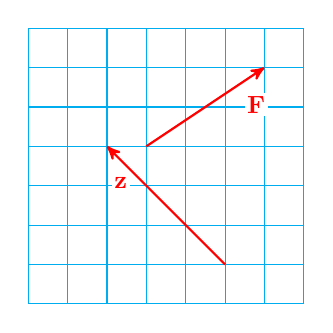
\begin{tikzpicture} [scale=.5]
\draw[cyan] (0,0) grid (7,7);
\coordinate (F) at (3,2);
\coordinate (z) at (-3,3);

\draw[red, thick,->,>=stealth'] (3,4)--++(F) node[below, xshift=-3,  yshift=-9, scale=.9, fill=white, inner sep=1]{\textbf{F}};
\draw[red, thick,->,>=stealth'] (5,1)--++(z) node[below , xshift=5, yshift=-10, scale=.9, fill=white, inner sep=1]{\textbf{z}};

\end{tikzpicture}
\newline


hp9-1-45 vectors on grid

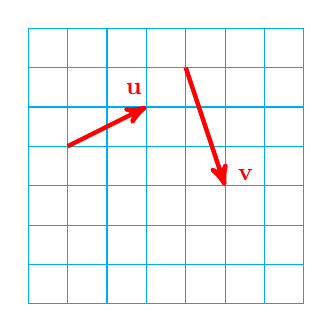
\begin{tikzpicture} [scale=.5]
\draw[cyan] (0,0) grid (7,7);
\coordinate (u) at (2,1);
\coordinate (v) at (1,-3);

\draw[red, ultra thick,->,>=stealth'] (4,6)--++(v) node[right, xshift=3, yshift=4, scale=.9, fill=white, inner sep=1]{\textbf{v}};
\draw[red, ultra thick,->,>=stealth'] (1,4)--++(u) node[above left, yshift=3, scale=.9, fill=white, inner sep=1]{\textbf{u}};

\end{tikzpicture}
\newline


hp9-1-45ans vectors on grid

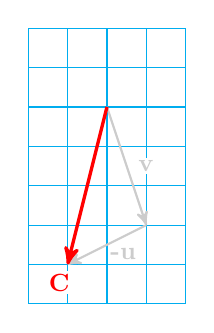
\begin{tikzpicture} [scale=.5]
\draw[cyan] (0,0) grid (4,7);
\coordinate (u) at (2,1);
\coordinate (v) at (1,-3);
\coordinate (C) at ($ (v) - (u) $);

\draw[lightgray!80!white, thick,->,>=stealth'] (2,5)--++(v) node[right, midway, xshift=3, scale=.9, fill=white, inner sep=1]{\textbf{v}};
\draw[lightgray!80!white, thick,->,>=stealth'] (3,2)--++($-1*(u)$) node[ below right, midway, scale=.9, fill=white, inner sep=1]{\textbf{-u}};
\draw[red,very thick,->,>=stealth'] (2,5)--++(C) node[below, xshift=-3, yshift=-2,  scale=.9, fill=white, inner sep=1]{\textbf{C}};

\end{tikzpicture}
\newline


hp9-1-46 vectors on grid

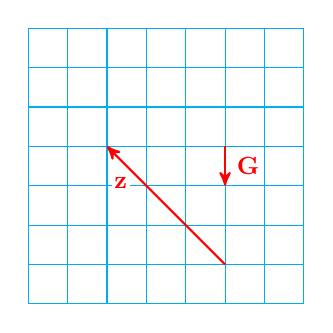
\begin{tikzpicture} [scale=.5]
\draw[cyan] (0,0) grid (7,7);
\coordinate (G) at (0,-1);
\coordinate (z) at (-3,3);

\draw[red, thick,->,>=stealth'] (5,4)--++(G) node[right, midway, xshift=3,  scale=.9, fill=white, inner sep=1]{\textbf{G}};
\draw[red, thick,->,>=stealth'] (5,1)--++(z) node[below , xshift=5, yshift=-10, scale=.9, fill=white, inner sep=1]{\textbf{z}};

\end{tikzpicture}
\newline


hp9-1-47 vectors on grid

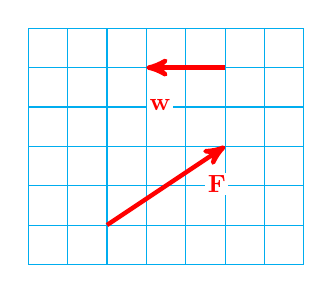
\begin{tikzpicture} [scale=.5]
\draw[cyan] (0,0) grid (7,6);
\coordinate (F) at (3,2);
\coordinate (w) at (-2,0);

\draw[red, ultra thick,->,>=stealth'] (2,1)--++(F) node[below, xshift=-3,  yshift=-9, scale=.9, fill=white, inner sep=1]{\textbf{F}};
\draw[red, ultra thick,->,>=stealth'] (5,5)--++(w) node[below , xshift=5, yshift=-10, scale=.9, fill=white, inner sep=1]{\textbf{w}};

\end{tikzpicture}
\newline


hp9-1-47ans vectors on grid

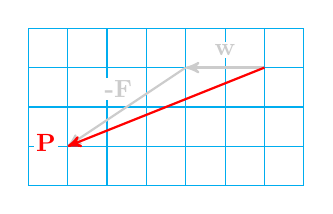
\begin{tikzpicture} [scale=.5]
\draw[cyan] (0,0) grid (7,4);
\coordinate (F) at (3,2);
\coordinate (w) at (-2,0);
\coordinate (P) at ($ (w) - (F) $);

\draw[lightgray!80!white,  thick,->,>=stealth'] (4,3)--++ ($-1*(F)$) node[above, midway, xshift=-3,  yshift=2, scale=.9, fill=white, inner sep=1]{\textbf{-F}};
\draw[lightgray!80!white,  thick,->,>=stealth'] (6,3)--++(w) node[above, midway, yshift=3, scale=.9, fill=white, inner sep=1]{\textbf{w}};
\draw[red, thick,->,>=stealth'] (6,3)--++(P) node[above left, xshift=-3, yshift=-3, scale=.9, fill=white, inner sep=1]{\textbf{P}};

\end{tikzpicture}
\newline


hp9-1-48 vectors on grid

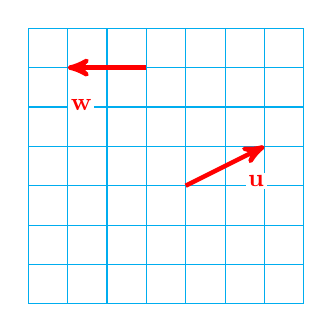
\begin{tikzpicture} [scale=.5]
\draw[cyan] (0,0) grid (7,7);
\coordinate (u) at (2,1);
\coordinate (w) at (-2,0);

\draw[red, ultra thick,->,>=stealth'] (4,3)--++(u) node[below, xshift=-3,  yshift=-9, scale=.9, fill=white, inner sep=1]{\textbf{u}};
\draw[red, ultra thick,->,>=stealth'] (3,6)--++(w) node[below , xshift=5, yshift=-10, scale=.9, fill=white, inner sep=1]{\textbf{w}};

\end{tikzpicture}
\newline


hp9-1-49 vectors on grid

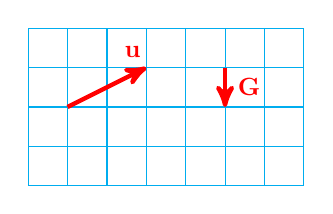
\begin{tikzpicture} [scale=.5]
\draw[cyan] (0,0) grid (7,4);
\coordinate (u) at (2,1);
\coordinate (G) at (0,-1);

\draw[red, ultra thick,->,>=stealth'] (1,2)--++(u) node[above, xshift=-5,  yshift=2, scale=.9, fill=white, inner sep=1]{\textbf{u}};
\draw[red, ultra thick,->,>=stealth'] (5,3)--++(G) node[right, midway, xshift=3, scale=.9, fill=white, inner sep=1]{\textbf{G}};

\end{tikzpicture}
\newline


hp9-1-49ans vectors on grid

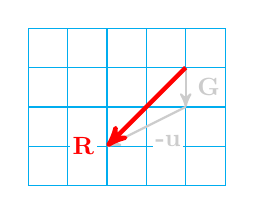
\begin{tikzpicture} [scale=.5]
\draw[cyan] (0,0) grid (5,4);
\coordinate (u) at (2,1);
\coordinate (G) at (0,-1);
\coordinate (R) at ($ (G) - (u)  $);

\draw[lightgray!80!white,  thick,->,>=stealth'] (4, 2)--++($-1*(u)$) node[below right, midway, xshift=2,  yshift=-2, scale=.9, fill=white, inner sep=1]{\textbf{-u}};
\draw[lightgray!80!white,  thick,->,>=stealth'] (4,3)--++(G) node[right, midway, xshift=3, scale=.9, fill=white, inner sep=1]{\textbf{G}};
\draw[red, ultra thick,->,>=stealth'] (4,3)--++(R) node[left , xshift=-3, scale=.9, fill=white, inner sep=1]{\textbf{R}};

\end{tikzpicture}
\newline


hp9-1-50 vectors on grid

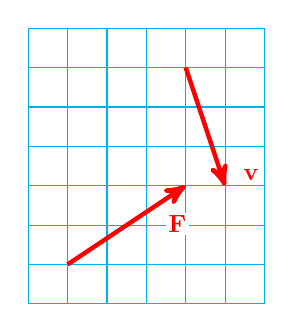
\begin{tikzpicture} [scale=.5]
\draw[cyan] (0,0) grid (6,7);
\coordinate (F) at (3,2);
\coordinate (v) at (1,-3);

\draw[red, ultra thick,->,>=stealth'] (1,1)--++(F) node[below, xshift=-3,  yshift=-9, scale=.9, fill=white, inner sep=1]{\textbf{F}};
\draw[red, ultra thick,->,>=stealth'] (4,6)--++(v) node[right , xshift=5, yshift=4, scale=.9, fill=white, inner sep=1]{\textbf{v}};

\end{tikzpicture}
\newline





\end{document}
